\documentclass{article} % For LaTeX2e
\usepackage{nips15submit_e,times}
\usepackage{hyperref}
\usepackage{url}
%\documentstyle[nips14submit_09,times,art10]{article} % For LaTeX 2.09

\usepackage{amsfonts}
\usepackage{float}
\usepackage{boxedminipage}
\usepackage{multirow}
\usepackage{pbox}
\usepackage{graphicx}

\newfloat{Algorithm}{hbtp}{lop}[section]
\newcommand{\etal}{{\it et al.}}
\newcommand{\eps}{\epsilon}
\newcommand{\veps}{\varepsilon}
\newcommand{\kmpp}{{\tt $k$-means++seed}}

\title{Fast Parallel Initialization for $k$-means \\
\tiny{PLEASE DO NOT DISTRIBUTE}}

\author{
Dipankar Das\\
Intel Labs Bangalore\\
\texttt{dipankar.das@intel.com} \\
\And
Jatin Garg \\
IIT Delhi \\
\texttt{cs1110223@cse.iitd.ac.in} \\
\AND
Sachin Goel \\
IIT Delhi \\
\texttt{cs1110249@cse.iitd.ac.in} \\
\And
Ragesh Jaiswal\thanks{Thanks to funding agencies.} \\\\
IIT Delhi \\
\texttt{rjaiswal@cse.iitd.ac.in} \\
\And
Sandeep Sen \\
IIT Delhi \\
\texttt{ssen@cse.iitd.ac.in}
}

% The \author macro works with any number of authors. There are two commands
% used to separate the names and addresses of multiple authors: \And and \AND.
%
% Using \And between authors leaves it to \LaTeX{} to determine where to break
% the lines. Using \AND forces a linebreak at that point. So, if \LaTeX{}
% puts 3 of 4 authors names on the first line, and the last on the second
% line, try using \AND instead of \And before the third author name.

\newcommand{\fix}{\marginpar{FIX}}
\newcommand{\new}{\marginpar{NEW}}

\nipsfinalcopy % Uncomment for camera-ready version

\begin{document}


\maketitle

\begin{abstract}
We provide a fast data-parallel initialization routine for $k$-means algorithm. 
The algorithm is based on sampling techniques that are easy to implement and parallelize. 
These parallel algorithms are implemented on a dual-socket Intel\textregistered Xeon\textregistered E5-2680v2. 
Empirical evaluations on large real and synthetic datasets demonstrates the practical utility of our techniques.
\end{abstract}

\section{Introduction}

\paragraph{$k$-means} Clustering is one of the most basic data processing tasks. 
So, any improvement in quality or efficiency in the popular clustering techniques has a significant impact.
We consider the $k$-means problem and the $k$-means algorithm (also known as the Lloyds algorithm) that are the one of the most popular clustering problems and solutions respectively, known in the Machine Learning literature.
The $k$-means problem is defined in the following manner: given a set of points $X \in \mathbb{R}^d$ and an integer $k$, find a set of centers $C \subset \mathbb{R}^d$ such that the cost 
$$\Phi_C(X) \stackrel{def.}{=} \sum_{x \in X} \min_{c \in C} ||x - c||^2$$ 
is minimized.
These $k$ centers induce a natural partition of the data points (points that are closest to the same center are in the same partition).
This is also known as the {\em Voronoi} partition.
The computational hardness of this problem is well understood and it is known that the problem is $\mathsf{NP}$-hard \cite{das08}.
Various approximation algorithms for this problem is known \cite{KanungoMNPSW02,charikar02}. 
However, the algorithm that is used to solve the $k$-means problem is practice is the $k$-means algorithm.\footnote{Unfortunately the algorithm has the same name as the problem. 
So, the reader should be careful while reading.}
This is a local search algorithm that starts with an arbitrary set of $k$ centers and then locally shifts these centers so that the cost of decreases and continue until no local improvement is possible.
Even though this algorithm gives good results in practice, the algorithm does not provide any guarantees in terms of performance or quality with respect to the the cost function.
This basically means that the $k$-means algorithm may take a huge amount of time to converge or the the solution produced has arbitrarily higher cost compared to the best solution. 
One way to ensure solution quality is to initialise the $k$-means algorithm with $k$ centers that satisfies some minimal quality guarantee. 
It is known that the $k$-means algorithm only improves the cost while execution. 
So, at the end, the quality guarantee follows from the initial centers.
In some sense, we get the best of both worlds -- $k$-means algorithm ensures good practical performance and initial centers ensures some minimal quality guarantee.

\noindent

\paragraph{Seeding} So now the question shifts to how to pick the initial centers for the $k$-means algorithm? 
This is sometimes known as the ``seeding" algorithm.
The requirements of such a seeding algorithm is that it should be (i) fast, (ii) simple, and (iii) give some quality guarantee.
\footnote{Simplicity is a subjective measure and hence data scientists might not be comfortable with such a requirement.
However, it is an important measure since simpler techniques have advantages when it comes to implementation and debugging.}
There has been a significant amount of work in obtaining algorithms that give quality guarantees. 
That is, obtaining approximation algorithms. 
So, as far as requirement (iii) is concerned, there are many candidate algorithms. 
However, most of these algorithms do not satisfy (i) and (ii).
One of the most popular algorithms that seem to satisfy all the properties and is popularly used as a seeding algorithm for the $k$-means algorithm is the \kmpp\ algorithm \cite{av07} that uses a simple sampling based approach. 
Here, the $k$ points are sampled in the following manner: Pick the first center uniformly at random and for $i > 1$, pick a point $p$ to be the $i^{th}$ center with probability proportional to the squared Euclidean distance of $p$ from the nearest center from among the set of previously chosen $(i-1)$ centers $C_{i-1}$ (i.e., with probability $\frac{\Phi_{C_{i-1}}(\{p\})}{\Phi_{C_{i-1}}(X)}$). 
This sampling procedure is also called the $D^2$-sampling~\cite{jks}.
Arthur and Vassilvitskii~\cite{av07} showed that this sampling procedure gives an approximation factor of $O(\log{k})$ in expectation.
This sampling based idea was further developed by Jaiswal \etal~\cite{jks} and they gave a sampling based algorithm that gives a solution that is arbitrarily close to the optimal solution in terms of the cost.
That is, they give a $(1 + \veps)$-approximation algorithm for arbitrary small $\veps$.
Moreover, their algorithm has another advantage that the algorithm has an inherent massively parallel version.
However, the running time of their algorithm is $O(nd \cdot 2^{\tilde{O}(k/\varepsilon}))$ which is large for practical relevance even with parallelisation. 
In this work, we explore a simple modified version of their algorithm with much smaller 
running time. 
Note that the strong approximation guarantee of the original algorithm is compromised in this process. 
However, through empirical analysis on large datasets we build some confidence that the quality of the solution produced is good.
We do extensive comparative analysis with the other seeding techniques.
The modified algorithm remains inherently parallel and we do a parallel implementation of our algorithm that we discuss next.
Note that the $k$-means algorithm runs in a number of rounds and these rounds are sequential.
So, if the seed $k$ centers result in smaller number of rounds and furthermore the seeding algorithm is parallel, then that means that we are effectively using the parallel architecture for $k$-means clustering. 
We also do a comparative analysis of the decrease in the number of rounds of the $k$-means algorithm (i.e., number of Lloyd iterations).

\paragraph{Parallel algorithm}
The parallel algorithms discussed in this work are designed for a shared memory parallel programming model, where all parallel computation threads/processes can view data written into the shared memory by any of the threads/processes.
Such shared-memory multi/many-core processors are widely available these days.
Designing parallel algorithms for important tasks such as clustering that exploit this readily available parallelism has gained importance.










\section{The Algorithm}
We start with a discussion of the algorithm of Jaiswal \etal\ \cite{jks} since our algorithm will be a modification of their algorithm.
Given a dataset $X$, let the optimal clusters be denoted by $X_1, ..., X_k$.
Suppose we have $i$ centers $C_i = \{c_1, ..., c_i\}$ such that these centers are good centers for some $i$ optimal clusters. 
That is, there exists distinct indices $j_1, ..., j_i \in \{1, ..., k\}$ such that $\forall l \leq i, \Phi_{c_l}(X_{j_l}) \leq (1 + O(\varepsilon)) \cdot \Delta(X_{j_l})$, where $\Delta(X_{j_l})$ denotes the optimal $1$-means cost of the cluster $X_{j_l}$.
Suppose at this time, we sample a set $S$ of $N$ points independently with the sampling technique of \kmpp. 
A formal description of \kmpp\ is given in Figure \ref{fig:kmpp}
Since the sampling technique gives preference to points that are further away from the current centers, we are likely to sample points from clusters whose indices do not appear in the set $\{j_1, ..., j_i\}$.
Let us call such clusters ``uncovered" clusters.
So, there is a good chance that a significant number of sampled points will be from uncovered clusters.
The algorithm of Jaiswal \etal\ \cite{jks} just considers all possible subset of points of size $M < N$ and considers the centroid of these points as the $(i+1)^{\textrm{th}}$ center. 
The main idea being that at least one of these subsets will behave as a uniform sample of points from some uncovered cluster and known results~\cite{inaba} suggests that the centroid of such a sample will be a good center for this uncovered cluster.
However, this results in the exponential running time since each time sampling is done, there are more than $1$ subsets to consider. 
\footnote{Even if we consider only two possibilities in each step, the running time will be $2^k$ since we have the sample $k$ times.}

\noindent
Our algorithm follows the same idea as that of Jaiswal~\etal\ \cite{jks} given in the above paragraph. 
However, while choosing the $(i+1)^{\textrm{th}}$ center, we do not try more than one possibility.
Instead of considering all possible subsets of $S$, we cluster $S$ into $k$ clusters using the \kmpp\ algorithm and then pick the centroid of the largest cluster as the $(i+1)^{th}$ center. 
\footnote{Ties are broken arbitrarily.}
Figure~\ref{fig:seed} gives a formal description of our algorithm. 
Figure~\ref{fig:illustration} gives an illustration of one iteration of our algorithm.
This algorithm has inherent data level parallelism. 
The parallel version of our algorithm is given in Figure~\ref{fig:par-seed}.
The rationale behind this choice for the $(i+1)^{th}$ center is the following: 
Let $X_l$ denote the uncovered cluster that is farthest from the current set $C_i$ of centers. That is, $\Phi_{C_i}(X_l)$ is the largest amongst the uncovered clusters. 
Note that $S$ is likely to have more points from $X_l$ than any other optimal cluster.
Ideally, we would like to isolate the points from $X_l$ present in $S$ and then take the centroid of these points. 
In Jaiswal~\etal\ \cite{jks} this was done by taking all possible subsets to ensure that one of these subsets contain all points from $X_l$. 
What we essentially do here is to cluster the points in $S$, the hope being that all points in $X_l$ that are present in $S$ will form a cluster.
Since our algorithm picks the largest cluster it would be able to isolate the points of $X_l$ present in $S$.

\noindent
Note that our suggested algorithm is a heuristic and we do not give any provable guarantees for our algorithm.
So, the only way to validate the effectiveness of our algorithm is to do a detailed experimental analysis on real and synthetic datasets. 
This is what we discuss in the remaining paper. 


\begin{center}
\begin{Algorithm}[h]
\begin{boxedminipage}{5.5in}
{\tt $D^2$-Seeding($X, k, N$)}

\hspace{0.1in} (1) $C_0 \leftarrow \{\}$

\hspace{0.1in} (2) For $i$ = $1$ to $k$

\hspace{0.3in} (a) Sample a multiset $S$ of $N$ points from $X$ using $D^2$ sampling with respect to $C_{i-1}$. \footnote{When $i=1$, $D^2$-sampling is the same as uniform sampling.}

\hspace{0.3in} (b) Let $T_l$ denote the largest cluster obtained by running \kmpp 

\hspace{0.3in}  \ \ \ \ \ \ algorithm on inputs $S$ and $k$.

\hspace{0.3in} (c) $c_i \leftarrow \Gamma(T_l)$ and $C_i \leftarrow C_{i-1} \cup \{c_i\}$. 
\footnote{$\Gamma(T)$ denote the centroid of the points in $T$ i.e., $\Gamma(T) = \frac{\sum_{t \in T} t}{|T|}$.}

\hspace{0.1in} (3) Output $C_k$
\end{boxedminipage}
\caption{Our seeding algorithm. $N$ is an input parameter that may be adjusted for performance/quality.}
\label{fig:seed}
\end{Algorithm}
\end{center}

\vspace{-0.4in}

\begin{center}
\begin{Algorithm}[h]
\begin{boxedminipage}{5.5in}
{\tt Par-$D^2$-Seeding($X, k, N$)}

\hspace{0.1in} (1) $C_0 \leftarrow \{\}$

\hspace{0.1in} (2) For all $1 \leq j \leq M$, let $P_j = \left\{X\left[{\frac{(j-1) \cdot |X|}{M}} \right], ..., X\left[{\frac{j \cdot |X|}{M}}\right]\right\}$. \footnote{$X[i]$ denotes the $i^{th}$ element of the dataset $X$}

\hspace{0.1in} (3) {\bf For} $i$ $\leftarrow$ $1$ to $k$:

%\hspace{0.3in} (a) {\bf Parfor} $j$ $\leftarrow$ $1$ to $M$

%\hspace{0.5in} (i) Sample a multiset $S_j$ of $N$ points from $P_j$ using $D^2$-sampling  with respect to $C_{i-1}$. 

\hspace{0.3in} (a) $S \leftarrow \{\}$ \ \ \ \ \ \ \ \ \ {\it // $S$ here denotes a multiset.}

\hspace{0.3in} (b) {\bf Parallel-for} $j \leftarrow 1$ to $M$:

\hspace{0.5in} (i) For all $1 \leq l \leq |X|/M$, $D_j[l] \leftarrow \Phi_{C_{i-1}}(\{P_j[l]\})$.

\hspace{0.5in} (ii) $D[j] \leftarrow \Phi_{C_{i-1}}(P_j)$.

\hspace{0.3in} (c) Let $\mathcal{D}$ denote the distribution over $\{1, ..., M\}$ defined by $D[1], ..., D[M]$.

\hspace{0.3in} (d) For all $j$, let $\mathcal{D}_j$ denote a distribution over $\left\{1, ..., \frac{|X|}{M} \right\}$ defined by $D_j[1], ..., D_j \left[\frac{|X|}{M}\right]$.


\hspace{0.3in} (e) {\bf Parallel-for} $j$ $\leftarrow$ $1$ to $N$:

\hspace{0.5in} (i) Sample $r$ from $\mathcal{D}$ and then $t$ from $\mathcal{D}_r$.

\hspace{0.5in} (ii) $S \leftarrow S \cup P_r[t]$.

\hspace{0.3in} (f) Let $T_l$ denote the largest cluster obtained by running \kmpp

\hspace{0.3in}  \ \ \ \ \ \ algorithm on inputs $S$ and $k$.

\hspace{0.3in} (g) $c_i \leftarrow \Gamma(T_l)$ and $C_i \leftarrow C_{i-1} \cup \{c_i\}$. 

\hspace{0.1in} (4) Output $C_k$
\end{boxedminipage}
\caption{Parallel version of our seeding algorithm. $N$ is an input parameter and $M$ is a global environment variable indicating the number of hardware-level threads available.}
\label{fig:par-seed}
\end{Algorithm}
\end{center}


\begin{figure}
\centering
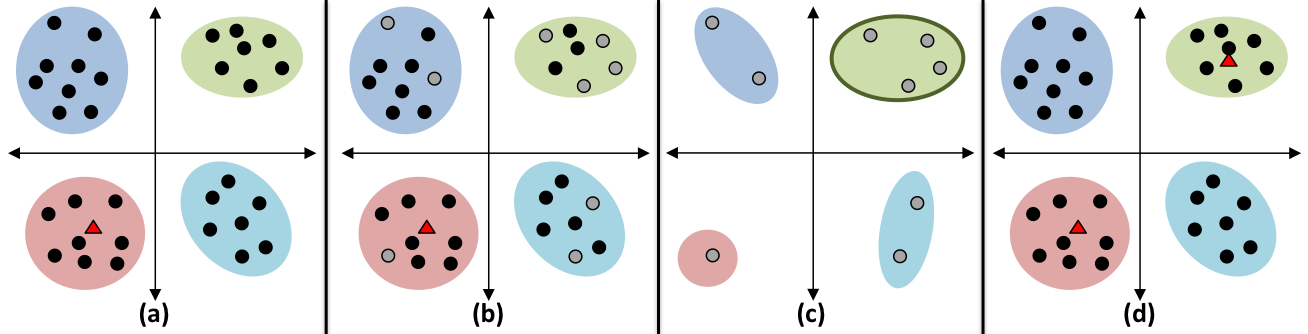
\includegraphics[scale=0.3]{illustration}
\caption{(a) First center (red triangle) has been chosen in iteration $1$ (b) Points (in gray) are sampled with $D^2$-sampling (c) The sampled points are clustered (d) Centroid of the largest cluster is chosen as the second center.}
\label{fig:illustration}
\end{figure}




\section{Experimental Analysis}

\subsection{Datasets and machine}
We use the following datasets for evaluating our algorithm.
Note that the first three datasets are real datasets and the last three are synthetically generated datasets.
The sequential algorithms in this work were implemented and evaluated on a single workstation with a dual-socket Intel\textregistered Xeon\textregistered E5-2680v2, with 20 cores and 40 threads, and operating at 2.8GHz running Ubuntu 14.04. We build our code using the GCC 4.8.2 and use OpenMP based thread parallelism.

\begin{table}[h]
\centering
\begin{tabular}{| l | l | c | c | c |}
\hline
{\bf Dataset} & {\bf Details} & $n$ & $d$ & $k$ \\
\hline \hline
MNIST & Handwriting dataset~\cite{mnist} & 70000 & 784 & 10 \\
\hline
CIFAR & CIFAR-10 Image dataset~\cite{cifar}  & 60000 & 3072 & 10 \\
\hline
3D & 3D Road Network dataset~\cite{3D} & 434874 & 3 & 5 \\
\hline
Birch1 & 2D Gaussians in a grid~\cite{birch} & 100000 & 2 & 100 \\
\hline
Birch2 & 2D Gaussians on a sine curve~\cite{birch} & 100000 & 2 & 100 \\
\hline
Birch3 & 2D Gaussians at random locations~\cite{birch} & 100000 & 2 & 100 \\
\hline
\end{tabular}
\caption{Datasets used for evaluation in this work.}
\end{table}





\subsection{Parameter $N$}
Before we start the comparative analysis, we would like to discuss the parameter $N$ of our \texttt{$D^2$-seeding} algorithm.
We will pick $N > k$.\footnote{This would avoid problems in step 2(b).
However, note that if $N \leq k$, then our algorithm is basically the \kmpp\ algorithm. 
This is because in each iteration, we pick a point sampled with $D^2$-sampling as the next center.
So, \kmpp\ algorithm is one of the extreme cases of our algorithm.}
How large should $N$ be as a function of $k$? Note that the larger the number of points from an uncovered cluster that we are able to isolate, the better is the centroid of these isolated points with respect to this uncovered cluster. 
The number of points from each uncovered cluster will be clearly larger for larger values of $N$.
However, the running time of the algorithm grows as $N$ increases. 
%Moreover, the ability of \kmpp\ to isolate the points in the most prominent uncovered cluster (in terms of current cost of clusters) might diminish with increasing number of sampled points.
So, there is a quality/performance tradeoff and the user should pick a value of $N$ that gives the best results.
We give cost analysis for values of $N$ that are multiples of $k$ in Table~\ref{table:2}.
Since our algorithm is randomized, we give the mean and standard deviation of the cost over $20$ runs over the datasets. 

We note that there is a significant improvement as $N$ is increased from $k$ to $10k$. 
However, the improvement is not that significant when comparing $N=10k$ and $N = 100k$.
We suggest using $N = 10k$ as a standard input for our algorithm. 
However, the user may adjust this parameter depending on the database for best performance. The supplementary material gives a finer grained analysis of cost w.r.t. $N$.

\begin{table}[h]
\centering
\begin{tabular}{| l | c | c | c | c | c | c | c |}
\hline
 $\mathbf{N}$ & & \pbox{2cm}{{\bf MNIST} \\\tiny($\times 10^{10}$)} & \pbox{2cm}{{\bf CIFAR} \\ \tiny{($\times 10^{10}$)}} & \pbox{2cm}{{\bf 3D} \\ \tiny{($\times 10^6$)}} & \pbox{2cm}{{\bf Birch1} \\ \tiny{($\times 10^{12}$)}} & \pbox{2cm}{{\bf Birch2} \\\tiny{($\times 10^{10}$)}} & \pbox{2cm}{{\bf Birch3} \\ \tiny{($\times 10^{12}$)}} \\
\hline \hline
\multirow{2}{*}{$k$} & mean & $32.39$ & $80.90$ & $15.98$ & $187.67$ & $158.02$ & $66.45$\\ \cline{2-8}
& \small{sd} & ${\scriptstyle 1.31}$ & ${\scriptstyle 6.11}$ & ${\scriptstyle 5.05}$ & ${\scriptstyle 7.88}$ & ${\scriptstyle 16.68}$ & ${\scriptstyle 3.47}$\\
\hline \hline 
\multirow{2}{*}{$10k$} & mean & $21.19$ & $53.92$ & $11.89$ & $120.39$ & $49.76$ & $45.35$\\ \cline{2-8}
& \small{sd} & ${\scriptstyle 4.45}$ & ${\scriptstyle 1.71}$ & ${\scriptstyle 2.71}$ & ${\scriptstyle 3.48}$ & ${\scriptstyle 1.16}$ & ${\scriptstyle 1.10}$\\
\hline \hline 
\multirow{2}{*}{$100k$} & mean & $21.18$ & $53.37$ & $11.51$ & $121.50$ & $50.30$ & $45.59$\\ \cline{2-8}
& \small{sd} & ${\scriptstyle 4.12}$ & ${\scriptstyle 1.37}$ & ${\scriptstyle 1.76}$ & ${\scriptstyle 3.41}$ & ${\scriptstyle 1.80}$ & ${\scriptstyle 1.09}$\\
\hline 
\end{tabular}
\caption{This table gives the cost of the solution produced by our seeding algorithm as a function of the input parameter $N$.}
\label{table:2}
\end{table}








\subsection{Cost, number of lloyds iterations, and running time}
Recall that for a given set $C$ of centers, the cost is given by $\Phi_{C}(X) = \sum_{x \in X} \min_{c \in C} ||x - c||^2$.
Given cost of the solution as an evaluation metric, we compare our algorithm with \kmpp\  which is widely believed to give the best results and is used in practice to obtain the seed for the $k$-means algorithm. 
For comparison purposes, we also give results for the \texttt{Random} procedure that picks $k$ centers uniformly at random and is the simplest seeding algorithm.
Since all the three procedures are randomized, we give the mean and standard deviation measured over $20$ runs. 
The cost comparison is given in Table~\ref{table:3}.
We note that the our algorithm (with $N=10k$) gives much better results compared to the other algorithms.

\begin{table}[h]
\centering
\begin{tabular}{| l | c | c | c | c | c | c | c |}
\hline
{\bf Algorithm} & & \pbox{2cm}{{\bf MNIST} \\\tiny($\times 10^{10}$)} & \pbox{2cm}{{\bf CIFAR} \\ \tiny{($\times 10^{10}$)}} & \pbox{2cm}{{\bf 3D} \\ \tiny{($\times 10^6$)}} & \pbox{2cm}{{\bf Birch1} \\ \tiny{($\times 10^{12}$)}} & \pbox{2cm}{{\bf Birch2} \\\tiny{($\times 10^{10}$)}} & \pbox{2cm}{{\bf Birch3} \\ \tiny{($\times 10^{12}$)}} \\
\hline \hline
\multirow{2}{*}{\small{\tt Random}} & mean & 
$31.99$ & $78.87$ & $55.32$ & $289.97$ & $713.26$ & $152.59$\\ \cline{2-8}
& \small{sd} & ${\scriptstyle 1.24}$ & ${\scriptstyle 4.81}$ & ${\scriptstyle 44.26}$ & ${\scriptstyle 30.91}$ & ${\scriptstyle 203.07}$ & ${\scriptstyle 26.17}$\\
\hline \hline 
\multirow{2}{*}{\tiny{\kmpp}} & mean & 
$32.03$ & $79.46$ & $15.66$ & $190.82$ & $167.57$ & $67.36$\\ \cline{2-8}
& \small{sd} & ${\scriptstyle 1.09}$ & ${\scriptstyle 6.17}$ & ${\scriptstyle 4.33}$ & ${\scriptstyle 7.68}$ & ${\scriptstyle 22.18}$ & ${\scriptstyle 4.65}$\\
\hline \hline 
\multirow{2}{*}{\pbox{5cm}{\small{\tt $D^2$-seeding} \\($N=k$)}} & mean & 
$32.39$ & $80.90$ & $15.98$ & $187.67$ & $158.02$ & $66.45$\\ \cline{2-8}
& \small{sd} & ${\scriptstyle 1.31}$ & ${\scriptstyle 6.11}$ & ${\scriptstyle 5.05}$ & ${\scriptstyle 7.88}$ & ${\scriptstyle 16.68}$ & ${\scriptstyle 3.47}$\\
\hline \hline 
\multirow{2}{*}{\pbox{5cm}{\small{\tt $D^2$-seeding} \\($N=10k$)}} & mean & 
$21.19$ & $53.92$ & $11.89$ & $120.39$ & $49.76$ & $45.35$\\ \cline{2-8}
& \small{sd} & ${\scriptstyle 0.44}$ & ${\scriptstyle 1.71}$ & ${\scriptstyle 2.71}$ & ${\scriptstyle 3.48}$ & ${\scriptstyle 1.16}$ & ${\scriptstyle 1.10}$\\
\hline \hline 
\multirow{2}{*}{\pbox{5cm}{\small{\tt $D^2$-seeding} \\($N=100k$)}} & mean & 
$21.18$ & $53.37$ & $11.51$ & $121.50$ & $50.30$ & $45.59$\\ \cline{2-8}
& \small{sd} & ${\scriptstyle 0.41}$ & ${\scriptstyle 1.37}$ & ${\scriptstyle 1.76}$ & ${\scriptstyle 3.41}$ & ${\scriptstyle 1.80}$ & ${\scriptstyle 1.09}$\\
\hline 
\end{tabular}
\caption{This table gives the cost of the solution produced by the seeding algorithms.}
\label{table:3}
\end{table}

We also compare cost of the solution obtained on running Lloyds iterations until convergence, post the seeding step.
The results of this comparison are given in Table~\ref{table:4}.
We note that for the synthetic datasets, we get a significant improvement. 
However, for the real datasets the final costs obtained are comparable.
Another interesting observation to be made when studying the experimental results in Tables~\ref{table:3} and \ref{table:4} is that cost of the solution produced by our seeding algorithm (with $N = 10k$) in Table~\ref{table:3} is consistently close to the best solution produced by the Lloyds algorithm in Table~\ref{table:4}.

\begin{table}[h]
\centering
\begin{tabular}{| l | c | c | c | c | c | c | c |}
\hline
{\bf Algorithm} & & \pbox{2cm}{{\bf MNIST} \\\tiny($\times 10^{10}$)} & \pbox{2cm}{{\bf CIFAR} \\ \tiny{($\times 10^{10}$)}} & \pbox{2cm}{{\bf 3D} \\ \tiny{($\times 10^6$)}} & \pbox{2cm}{{\bf Birch1} \\ \tiny{($\times 10^{12}$)}} & \pbox{2cm}{{\bf Birch2} \\\tiny{($\times 10^{10}$)}} & \pbox{2cm}{{\bf Birch3} \\ \tiny{($\times 10^{12}$)}} \\
\hline \hline
\multirow{2}{*}{\small{\tt Random}} & mean & 
$17.93$ & $47.43$ & $8.82$ & $111.75$ & $159.36$ & $49.33$\\ \cline{2-8}
& \small{sd} & ${\scriptstyle 0.0562}$ & ${\scriptstyle 0.0599}$ & ${\scriptstyle 0.0001}$ & ${\scriptstyle 5.8873}$ & ${\scriptstyle 21.6450}$ & ${\scriptstyle 5.4267}$\\
\hline \hline 
\multirow{2}{*}{\tiny{\kmpp}} & mean & 
$17.90$ & $47.46$ & $8.82$ & $106.24$ & $84.49$ & $40.41$\\ \cline{2-8}
& \small{sd} & ${\scriptstyle 0.0556}$ & ${\scriptstyle 0.1048}$ & ${\scriptstyle 0.0004}$ & ${\scriptstyle 3.4275}$ & ${\scriptstyle 8.8590}$ & ${\scriptstyle 1.3834}$\\
\hline \hline 
\multirow{2}{*}{\pbox{5cm}{\small{\tt $D^2$-seeding} \\($N=k$)}} & mean & 
$17.93$ & $47.45$ & $8.82$ & $106.31$ & $84.56$ & $40.45$\\ \cline{2-8}
& \small{sd} & ${\scriptstyle 0.0546}$ & ${\scriptstyle 0.0711}$ & ${\scriptstyle 0.0005}$ & ${\scriptstyle 3.3346}$ & ${\scriptstyle 10.6210}$ & ${\scriptstyle 1.0226}$\\
\hline \hline 
\multirow{2}{*}{\pbox{5cm}{\small{\tt $D^2$-seeding} \\($N=10k$)}} & mean & 
$17.91$ & $47.46$ & $8.82$ & $98.11$ & $45.67$ & $38.95$\\ \cline{2-8}
& \small{sd} & ${\scriptstyle 0.0706}$ & ${\scriptstyle 0.0667}$ & ${\scriptstyle 0.0005}$ & ${\scriptstyle 2.1194}$ & ${\scriptstyle 3.8557}$ & ${\scriptstyle 0.5371}$\\
\hline \hline 
\multirow{2}{*}{\pbox{5cm}{\small{\tt $D^2$-seeding} \\($N=100k$)}} & mean & 
$17.90$ & $47.44$ & $8.82$ & $97.58$ & $45.88$ & $39.02$\\ \cline{2-8}
& \small{sd} & ${\scriptstyle 0.0445}$ & ${\scriptstyle 0.0606}$ & ${\scriptstyle 0.0005}$ & ${\scriptstyle 2.3682}$ & ${\scriptstyle 0.94}$ & ${\scriptstyle 0.54}$\\
\hline 
\end{tabular}
\caption{This table gives the cost of the solution produced by the Lloyds algorithm with the initial centers obtained using the above seeding algorithms.}
\label{table:4}
\end{table}

Since our goal is to use our algorithm as a seeding algorithm for the $k$-means algorithm which is inherently sequential, the number of iterations of Lloyds algorithm that need to be run for convergence is an important metric. 
We say that the $k$-means algorithm has converged if the decrease in the cost is less than $0.0001$ times the current cost.
We do a comparative analysis of the number of Lloyds iterations.
The results of this comparison is given in Table~\ref{table:5}.
We note that our algorithm (with $N=10k$) gives improvements for all datasets.
These improvements are significant for the synthetic Birch datasets whereas the improvements are small for the real datasets.

\begin{table}[h]
\centering
\begin{tabular}{| l | c | c | c | c | c | c | c |}
\hline
{\bf Algorithm} & & {\bf MNIST} & {\bf CIFAR} & {\bf 3D} & {\bf Birch1} & {\bf Birch2} & {\bf Birch3} \\
\hline \hline
\multirow{2}{*}{\small{\tt Random}} & mean & 
$19.48$ & $22.32$ & $32.38$ & $41.54$ & $19.56$ & $51.78$\\ \cline{2-8}
& \small{sd} & ${\scriptstyle 7.94}$ & ${\scriptstyle 6.51}$ & ${\scriptstyle 6.25}$ & ${\scriptstyle 15.82}$ & ${\scriptstyle 9.06}$ & ${\scriptstyle 16.74}$\\
\hline \hline 
\multirow{2}{*}{\tiny{\kmpp}} & mean & 
$22.14$ & $24.18$ & $23.18$ & $30.28$ & $16.30$ & $41.78$\\ \cline{2-8}
& \small{sd} & ${\scriptstyle 6.60}$ & ${\scriptstyle 7.40}$ & ${\scriptstyle 10.04}$ & ${\scriptstyle 12.05}$ & ${\scriptstyle 6.55}$ & ${\scriptstyle 12.67}$\\
\hline \hline 
\multirow{2}{*}{\pbox{5cm}{\small{\tt $D^2$-seeding} \\($N=k$)}} & mean & 
$20.28$ & $23.18$ & $21.2$ & $30.46$ & $13.46$ & $40.32$\\ \cline{2-8}
& \small{sd} & ${\scriptstyle 6.52}$ & ${\scriptstyle 7.53}$ & ${\scriptstyle 8.98}$ & ${\scriptstyle 10.05}$ & ${\scriptstyle 5.21}$ & ${\scriptstyle 10.76}$\\
\hline \hline 
\multirow{2}{*}{\pbox{5cm}{\small{\tt $D^2$-seeding} \\($N=10k$)}} & mean & 
$20.88$ & $23.36$ & $20.12$ & $13.92$ & $2.42$ & $32.58$\\ \cline{2-8}
& \small{sd} & ${\scriptstyle 7.47}$ & ${\scriptstyle 6.90}$ & ${\scriptstyle 7.65}$ & ${\scriptstyle 7.66}$ & ${\scriptstyle 0.49}$ & ${\scriptstyle 10.35}$\\
\hline \hline 
\multirow{2}{*}{\pbox{5cm}{\small{\tt $D^2$-seeding} \\($N=100k$)}} & mean & 
$23.26$ & $21.88$ & $16.8$ & $12.20$ & $3.00$ & $33.90$\\ \cline{2-8}
& \small{sd} & ${\scriptstyle 8.06}$ & ${\scriptstyle 7.55}$ & ${\scriptstyle 6.68}$ & ${\scriptstyle 5.41}$ & ${\scriptstyle 0.79}$ & ${\scriptstyle 7.75}$\\
\hline 
\end{tabular}
\caption{This table gives the number of lloyds steps until convergence when the algorithm is executed with the seed produced by the above algorithms.}
\label{table:5}
\end{table}

We also do a running time comparison of the three algorithms.
The results are given in Table~\ref{table:6}.
Since our algorithm does more sampling work than \kmpp, the running time of our algorithm is of course larger. 
However, one should note that the running time is not more than twice as that of the \kmpp\ algorithm.

\begin{table}[h]
\centering
\begin{tabular}{| l | c | c | c | c | c | c | c |}
\hline
{\bf Algorithm} & & {\bf MNIST} & {\bf CIFAR} & {\bf 3D} & {\bf Birch1} & {\bf Birch2} & {\bf Birch3} \\
\hline \hline
\multirow{2}{*}{\small{\tt Random}} & mean & 
$0.0015$ & $0.0009$ & $0.0071$ & $0.0032$ & $0.0031$ & $0.0030$\\ \cline{2-8}
& \small{sd} & ${\scriptstyle 0.0004}$ & ${\scriptstyle 0.0001}$ & ${\scriptstyle 0.0009}$ & ${\scriptstyle 0.0005}$ & ${\scriptstyle 0.0007}$ & ${\scriptstyle 0.0005}$\\
\hline \hline 
\multirow{2}{*}{\tiny{\kmpp}} & mean & 
$29.8301$ & $96.0875$ & $1.8191$ & $136.9317$ & $133.9361$ & $134.245$\\ \cline{2-8}
& \small{sd} & ${\scriptstyle 0.2941}$ & ${\scriptstyle 0.6122}$ & ${\scriptstyle 0.1252}$ & ${\scriptstyle 0.4061}$ & ${\scriptstyle 0.3542}$ & ${\scriptstyle 0.4413}$\\
\hline \hline 
\multirow{2}{*}{\pbox{5cm}{\small{\tt $D^2$-seeding} \\($N=k$)}} & mean & 
$29.8118$ & $96.6231$ & $1.8755$ & $152.0806$ & $149.1547$ & $149.36$\\ \cline{2-8}
& \small{sd} & ${\scriptstyle 0.3951}$ & ${\scriptstyle 0.6524}$ & ${\scriptstyle 0.1060}$ & ${\scriptstyle 0.4001}$ & ${\scriptstyle 0.4189}$ & ${\scriptstyle 0.3795}$\\
\hline \hline 
\multirow{2}{*}{\pbox{5cm}{\small{\tt $D^2$-seeding} \\($N=10k$)}} & mean & 
$30.2519$ & $98.0837$ & $1.8372$ & $274.9108$ & $271.5379$ & $272.50$\\ \cline{2-8}
& \small{sd} & ${\scriptstyle 0.3230}$ & ${\scriptstyle 0.4534}$ & ${\scriptstyle 0.1325}$ & ${\scriptstyle 0.5928}$ & ${\scriptstyle 0.4878}$ & ${\scriptstyle 0.6575}$\\
\hline \hline 
\multirow{2}{*}{\pbox{5cm}{\small{\tt $D^2$-seeding} \\($N=100k$)}} & mean & 
$34.6420$ & $115.7657$ & $1.9183$ & $1509.3000$ & $1545.4000$ & $1511.4000$\\ \cline{2-8}
& \small{sd} & ${\scriptstyle 0.4269}$ & ${\scriptstyle 0.6319}$ & ${\scriptstyle 0.1915}$ & ${\scriptstyle 20.5850}$ & ${\scriptstyle 28.8680}$ & ${\scriptstyle 20.8380}$\\
\hline 
\end{tabular}
\caption{Running time (in seconds) of {\tt $D^2$-seeding}.}
\label{table:6}
\end{table}

\subsection{Parallel implementation and $M$}
Consider \texttt{Par-$D^2$-seeding}, the parallel version of our algorithm.
$M$ denotes the number of parallel threads executed.
The parallel steps in the algorithm are steps 3(b) and 3(e). 
We do an analysis of the running time as a function of the number of threads used in this parallel step.
The maximum number of threads in our analysis is $40$ since that is the total number of  hardware level threads available in the architecture that we use. 
This is just to understand the behaviour of our algorithm in terms of the amount of parallelism available.

\begin{table}[h]
\centering
\begin{tabular}{| l | c | c | c | c | c | c | c |}
\hline
{\bf \# Machines} & & {\bf MNIST} & {\bf CIFAR} & {\bf 3D} & {\bf Birch1} & {\bf Birch2} & {\bf Birch3} \\
\hline \hline
\multirow{2}{*}{$M=1$} & mean & 
$30.25$ & $98.08$ & $1.83$ & $274.91$ & $271.53$ & $272.50$\\ \cline{2-8}
& \small{sd} & ${\scriptstyle 0.32}$ & ${\scriptstyle 0.45}$ & ${\scriptstyle 0.13}$ & ${\scriptstyle 0.59}$ & ${\scriptstyle 0.48}$ & ${\scriptstyle 0.65}$\\
\hline \hline 
\multirow{2}{*}{$M=5$} & mean & 
$7.02$ & $22.31$ & $0.99$ & $152.64$ & $151.73$ & $155.62$\\ \cline{2-8}
& \small{sd} & ${\scriptstyle 1.19}$ & ${\scriptstyle 2.28}$ & ${\scriptstyle 0.20}$ & ${\scriptstyle 5.98}$ & ${\scriptstyle 5.72}$ & ${\scriptstyle 6.04}$\\
\hline \hline 
\multirow{2}{*}{$M = 10$} & mean & 
$3.53$ & $11.05$ & $0.56$ & $87.51$ & $87.22$ & $86.47$\\ \cline{2-8}
& \small{sd} & ${\scriptstyle 0.55}$ & ${\scriptstyle 0.49}$ & ${\scriptstyle 0.06}$ & ${\scriptstyle 3.81}$ & ${\scriptstyle 4.93}$ & ${\scriptstyle 3.66}$\\
\hline \hline 
\multirow{2}{*}{$M = 20$} & mean & 
$3.67$ & $8.53$ & $0.35$ & $46.77$ & $47.53$ & $48.04$\\ \cline{2-8}
& \small{sd} & ${\scriptstyle 1.27}$ & ${\scriptstyle 2.45}$ & ${\scriptstyle 0.06}$ & ${\scriptstyle 2.07}$ & ${\scriptstyle 2.37}$ & ${\scriptstyle 1.87}$\\
\hline \hline 
\multirow{2}{*}{$M=40$} & mean & 
$2.26$ & $6.72$ & $0.27$ & $37.16$ & $36.51$ & $38.50$\\ \cline{2-8}
& \small{sd} & ${\scriptstyle 0.60}$ & ${\scriptstyle 0.77}$ & ${\scriptstyle 0.06}$ & ${\scriptstyle 1.26}$ & ${\scriptstyle 1.35}$ & ${\scriptstyle 1.52}$\\
\hline 
\end{tabular}
\caption{Running time (in seconds) of \texttt{Par-$D^2$-seeding} as a function of $M$. $N$ is set to be $10k$.}
\end{table}

\paragraph{Parallel architecture} The {\tt Par-$D^{2}$-seeding} algorithm and other parallel algorithms discussed in this work are designed for a shared memory parallel programming model, where all parallel computation threads/processes can view data written into the shared memory by any of the threads/processes.
Examples of such systems are shared-memory multi-/many-core processors like Intel\textregistered Xeon\textregistered CPUs and Xeon Phi\texttrademark  coprocessors, and distributed shared memory systems like those using global arrays and partitioned global address space (PGAS) (\url{http://www.pgas.org}).    
In this work we implement the algorithms and conduct experiments on an Intel\textregistered Xeon\textregistered E5-2680v2 processor which supports upto 40 concurrent threads programmed by C++/OpenMP. 
The machine has $2$ sockets each with $10$ cores. Each core can support $2$ hyperthreads. 
So, the machine has effectively $20$ cores and $40$ threads. 
Note that this is the reason for a disproportionate running time decrease when $M$ increases from $20$ to $40$.
Moreover there is a serial segment in our algorithm since we choose not to parallelize step 3(f) (\kmpp\ step), and this becomes significant when $k$ (and hence $N$) is large as in case of Birch data-sets. 
Hence we do not witness linear scaling with increase in number of threads.
Finally, we believe that the algorithms proposed in this work are generic and applicable to any other system having shared memory parallelism, and can be easily extended to a message passing paradigm as well.





















\subsection{Analysis of \texttt{Par-$D^2$-Seeding}}
As far as parallel seeding algorithms for $k$-means is concerned, the most notable and recent algorithm is the {\tt $k$-means$||$} algorithm of Bahmani~\etal~\cite{bahmani}.
We compare the running time and cost of our parallel algorithm with parallel version of \kmpp, and \texttt{$k$-means$||$}. 
The pseudocodes for \kmpp\ and its parallel version are are given in Algorithm~\ref{fig:kmpp}. 
Algorithm~\ref{fig:scalable} gives the formal description of the {\tt $k$-means$||$} (Algorithm 2 in \cite{bahmani}) customised for our parallel setting.

\renewcommand{\sp}{{\hspace*{1 mm}}}
\newcommand{\append}{{\tt append}}
\newcommand{\pr}{\mathbf{Pr}}

  \begin{Algorithm}[ht]
    \begin{boxedminipage}{0.40\linewidth}
      {\kmpp(X, k)} : \medskip\\
       \sp \sp 1. $C_0 \leftarrow \{\}$ \\ 
       \sp \sp 2. {\bf For} $i$ $\leftarrow$ $1$ to $k$ \\
       \sp \sp \sp \sp \sp (a)  Sample a point $p$ from $X$ using \\
       \sp \sp \sp \sp \sp \sp \sp \sp \sp $D^2$-sampling w.r.t. $C_{i-1}$\\
       \sp \sp \sp \sp \sp (b)  $c_i \leftarrow p$; $C_{i} \leftarrow C_{i-1} \cup \{c_i\}$\\
       \sp \sp 3. Return $C_k$ \\\\\\\\\\\\\\
      \end{boxedminipage}      
       \begin{boxedminipage}{0.59\linewidth}
     {\bf {\tt Par-$k$-means++(X, k)} :} \medskip\\
       \sp \sp 1. $C_0 \leftarrow \{\}$ \\ 
       \sp \sp 2. Let $P_j = \left\{X\left[{\frac{(j-1)|X|}{M}}\right], ..., X\left[{\frac{j|X|}{M}}\right]\right\}$ for all $j$\\
       \sp \sp 3. {\bf For} $i$ $\leftarrow$ $1$ to $k$ \\
       \sp \sp \sp \sp \sp (a) {\bf Parallel-for} $j$ $\leftarrow$ $1$ to $M$ \\
       \sp \sp \sp \sp \sp \sp \sp \sp \sp \sp (i)  Sample a point $p_j$ from $P_j$ using $D^2$-sampling\\
       \sp \sp \sp \sp \sp \sp \sp \sp \sp \sp \sp \sp \sp  w.r.t. $C_{i-1}$\\
       \sp \sp \sp \sp \sp (b) Let $D$ denote the distribution over $\{1, ..., M\}$ s.t.\\
       \sp \sp \sp \sp \sp \sp \sp \sp \sp \sp $\pr[j \leftarrow D] = \frac{\Phi_{C_{i-1}}\left(P_j\right)}{\Phi_{C_{i-1}}(X)}$\\
       \sp \sp \sp \sp \sp (c) Sample $j$ from $D$ \\
       \sp \sp \sp \sp \sp (d) $c_i \leftarrow p_j$; $C_{i} \leftarrow C_{i-1} \cup \{c_{i}\}$\\
       \sp \sp 4. Return $C_k$
      \end{boxedminipage} 
      \caption{The \kmpp\ and {\tt Par-$k$-means++} algorithms. In the parallel implementation, $M$ indicates the number of hardware level threads available.}
       \label{fig:kmpp}
    \end{Algorithm}



\begin{center}
\begin{Algorithm}[ht]
\begin{boxedminipage}{5.6in}
{\tt $k$-means$||$($X, k, \ell, r$)}

\hspace{0.1in} (1) $C \leftarrow $ sample a point uniformly at random from $X$.

\hspace{0.1in} (2) {\bf For} $i \leftarrow $ $1$ to $r$:

\hspace{0.3in} (a) $S \leftarrow \{\}$. \ \ \ \ {\it $S$ is a multiset.}

\hspace{0.3in} (b) Use data-level parallelism as in step 3(b) of {\tt Par-$D^2$-seeding} to compute $\Phi_C(\{p\})$ $\forall p$.

\hspace{0.3in} (c) {\bf Parallel-for} $j$ $\leftarrow$ $1$ to $|X|$:
 
 \hspace{0.5in} (i) Add point $X[j]$ to $S$ with with probability  $\frac{\ell \cdot \Phi_{C}\left( \{X[j]\}\right)}{\Phi_C(X)}$.

\hspace{0.3in} (d) $C \leftarrow C \cup S$.

\hspace{0.1in} (5) For each $c \in C$ compute the weight of $c$ as the number of points in $X$ that has $c$ as the

\hspace{0.3in}  closest center in $C$.

\hspace{0.1in} (6) Cluster the weighted set $C$ using a weighted version of \kmpp\ and output the 

\hspace{0.3in} resulting $k$ centers.
\end{boxedminipage}
\caption{The {\tt $k$-means$||$} algorithm customized for our parallel setting. Recommended values~\cite{bahmani} of $\ell$ and $r$ are $\ell = 2k$ and $r=5$. $M$ indicates the number of parallel threads available.}
\label{fig:scalable}
\end{Algorithm}
\end{center}

\vspace{-0.5in}

The experimental results doing a comparison of cost and running time is given in Table~\ref{table:8}.
We note that our algorithm does significantly better with respect to the cost. 
As far as running time is concerned, on the real datasets our algorithm runs faster and this is reversed for the Birch datasets. 
This is due to large values of $k$ in the Birch datasets.
Note that our algorithm runs in $k$ iterations that are inherently sequential. 
This property is also present in the \kmpp\ algorithm.
{\tt $k$-means$||$} was designed precisely to remove this sequential iteration of length $k$ from \kmpp.
So, it is not surprising that whenever the value of $k$ is large, the {\tt $k$-means$||$} algorithm will run faster. 
However, our algorithm is more targeted towards getting a better quality solution which can also be seen from our experimental results.

\begin{table}[h]
\centering
\begin{tabular}{| l | c | c | c || c | c || c | c |}
\hline
& & \multicolumn{2}{ c |}{{\bf MNIST}} & \multicolumn{2}{ c |}{{\bf CIFAR}} & \multicolumn{2}{ c |}{{\bf 3D}} \\ \cline{3-8}
{\bf Algorithm} & & \pbox{1cm}{Cost\\\tiny{($\times 10^{10}$)}} & \pbox{1cm}{Time\\ \tiny(in sec.)} & \pbox{1cm}{Cost\\\tiny{($\times 10^{10}$)}} & \pbox{1cm}{Time\\ \tiny(in sec.)} & \pbox{1cm}{Cost\\\tiny{($\times 10^6$)}} & \pbox{1cm}{Time\\ \tiny(in sec.)}\\
\hline \hline
\multirow{2}{*}{\small{\tt Par-$k$-means++}} & mean & 
$32.42$ & $1.91$ & $80.45$ & $5.68$ & $17.82$ & $0.25$\\ \cline{2-8}
& \small{sd} & ${\scriptstyle 1.16}$ & ${\scriptstyle 0.51}$ & ${\scriptstyle 6.43}$ & ${\scriptstyle 0.47}$ & ${\scriptstyle 6.36}$ & ${\scriptstyle 0.03}$\\
\hline \hline 
%
\multirow{2}{*}{\pbox{5cm}{\small{\tt $k$-means$||$} \\ \tiny{($\ell=2k$, $r=5$)}}} & mean & 
$31.21$ & $10.68$ & $68.55$ & $34.29$ & $15.72$ & $2.92$\\ \cline{2-8}
& \small{sd} & ${\scriptstyle 1.02}$ & ${\scriptstyle 1.28}$ & ${\scriptstyle 2.89}$ & ${\scriptstyle 3.51}$ & ${\scriptstyle 5.06}$ & ${\scriptstyle 0.48}$\\
\hline \hline 
%
\multirow{2}{*}{\pbox{5cm}{\small{\tt Par-$D^2$-Seeding} \\ \tiny($N=10k$)}} & mean & 
$21.23$ & $2.26$ & $53.80$ & $6.72$ & $11.98$ & $0.27$\\ \cline{2-8}
& \small{sd} & ${\scriptstyle 0.49}$ & ${\scriptstyle 0.60}$ & ${\scriptstyle 1.33}$ & ${\scriptstyle 0.77}$ & ${\scriptstyle 2.02}$ & ${\scriptstyle 0.06}$\\
\hline
\end{tabular}
%\newline
%\vspace*{0.2cm}
%\newline
\bigskip
\vspace*{0.01cm}
\noindent
\begin{tabular}{| l | c | c | c || c | c || c | c |}
\hline
& & \multicolumn{2}{ c |}{{\bf Birch1}} & \multicolumn{2}{ c |}{{\bf Birch2}} & \multicolumn{2}{ c |}{{\bf Birch3}} \\ \cline{3-8}
{\bf Algorithm} & & \pbox{1cm}{Cost\\\tiny{($\times 10^{12}$)}} & \pbox{1cm}{Time\\ \tiny(in sec.)} & \pbox{1cm}{Cost\\\tiny{($\times 10^{10}$)}} & \pbox{1cm}{Time\\ \tiny(in sec.)} & \pbox{1cm}{Cost\\\tiny{($\times 10^{12}$)}} & \pbox{1cm}{Time\\ \tiny(in sec.)}\\
\hline \hline
\multirow{2}{*}{\small{\tt Par-$k$-means++}} & mean & 
$189.54$ & $27.39$ & $165.16$ & $26.83$ & $67.78$ & $25.55$\\ \cline{2-8}
& \small{sd} & ${\scriptstyle 8.76}$ & ${\scriptstyle 2.33}$ & ${\scriptstyle 21.25}$ & ${\scriptstyle 2.27}$ & ${\scriptstyle 4.72}$ & ${\scriptstyle 3.24}$\\
\hline \hline 
%
\multirow{2}{*}{\pbox{5cm}{\small{\tt $k$-means$||$} \\ \tiny{($\ell=2k$, $r=5$)}}} & mean & 
$190.09$ & $9.93$ & $156.26$ & $10.15$ & $67.73$ & $10.21$\\ \cline{2-8}
& \small{sd} & ${\scriptstyle 10.86}$ & ${\scriptstyle 0.65}$ & ${\scriptstyle 20.28}$ & ${\scriptstyle 0.72}$ & ${\scriptstyle 3.43}$ & ${\scriptstyle 0.76}$\\
\hline \hline 
%
\multirow{2}{*}{\pbox{5cm}{\small{\tt Par-$D^2$-Seeding} \\ \tiny{($N=10k$)}}} & mean & 
$120.63$ & $37.16$ & $50.40$ & $36.51$ & $45.66$ & $38.50$\\ \cline{2-8}
& \small{sd} & ${\scriptstyle 8.76}$ & ${\scriptstyle 2.33}$ & ${\scriptstyle 1.84}$ & ${\scriptstyle 1.35}$ & ${\scriptstyle 1.09}$ & ${\scriptstyle 1.52}$\\
\hline
\end{tabular}
\caption{Running time and cost for parallel algorithms. The number of machine threads used is $M = 40$.}
\label{table:8}
\end{table}



\vspace{-0.2in}

\section{Conclusion}
We suggest an initialization heuristic for $k$-means obtained by a suitable modification of  the sampling based algorithm of Jaiswal \etal~\cite{jks}.
Sampling based algorithms, apart from being simple, have the advantage the they are inherently parallel.
We give a parallel implementation of our algorithm.
We do a comparative analysis on large real and synthetic datasets comparing our results with the state-of-art algorithms.
Our experiments show notable cost and running time benefits.
We would like to recommend our algorithm as an alternative for the \kmpp\ algorithm as an initialization algorithm on any standard multicore platform since our algorithm exploits the available parallelism easily and efficiently to give very good quality solutions.

%\newpage


\bibliographystyle{plain}
{\footnotesize \bibliography{biblio}}

\end{document}
